\section{modélisation de la base de données}
la modélisation de la base de données s'est fait progressivement tout au long du stage. Chaque fois on essayait de l'améliorer en y apportant les ajouts nécessaire pour la faire correspondre à l'idée de départ, d'une base de données générique. Au moment de la rédaction du rapport, sa modélisation n'est pas encore fini ou plutôt n'est pas encore validé. Toute fois, nous avons décidé d'y insérer des données et la testée jusqu'à ce qu'à ce que nous rencontrions un problème.
\subsection{Principe d'une base de données générique}
D'une manière générale, lorsqu'on modélise une base de données, on regroupe entre eux les objets ayant les mêmes propriétés dans entités. Ainsi par exemple pour une base de données qui stocke des objets de type moutons et voitures, on aura des entités(tables) moutons et voiture comme dans l'exemple qui suit : 

\begin{figure}[h!]
\begin{center}
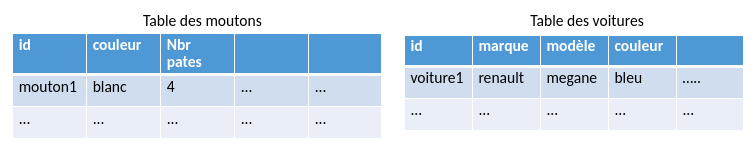
\includegraphics[width=1\textwidth]{images/bd_image1.png}
\end{center}
\caption{exemples de tables d'une base de données}
\label{exemples de tables d'une base de données}
\end{figure}

la modélisation devient d'autant plus difficile si dès le départ on ne connaît pas l'ensemble des objets que l'on doit stocker. En d'autres mots, on souhaite faire une base de données pour contenir plusieurs type d'objets dont les propriétés ne sont pas connu à l'avance. Dans l'exemple ci-dessus, ça correspondrait à stoker, en plus des moutons et des voitures, des immeubles, des personnes et tout autre type d'objet. Pour y remédier, on fait intervenir les bases de données générique. Cela consiste modifier la structure de notre entité et la faire correspondre à une système proche du schéma (clé:valeur). Ce cas de figure fait passer les propriétés des entités dans les colonnes.
l'exemple ci-dessous illustre bien ces propos

\begin{figure}[h!]
    \begin{center}
    \label{exemple de table d'une base de données générique}
         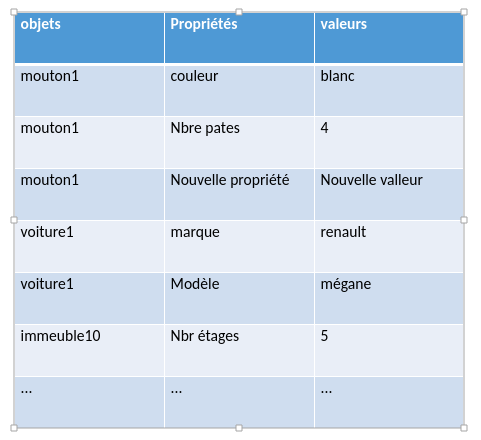
\includegraphics[width=0.4\textwidth]{images/bd_image2.png}
    \caption{exemple de table d'une base de données générique}
    \end{center}
\end{figure}


\subsubsection{Modélisation}
La valeur d'une donnée en générale et d'une donnée capteur émanant d'une mesure en particulier est d'autant plus important que celle-ci fait apparaître la dimension espace et la dimension temps.
A quoi nous servirait par exemple d'avoir 30$^\circ$ celsius, si on ne se pas à quel endroit fait référence à cette mesure ni à quelle moment elle a été relevé. Ce principe nous a guidé dans la modélisation de la base de données.
Pour faire intervenir la dimension espace, on s'est dit qu'un capteur est localisé dans un noeud et un noeud est un point d'un réseau de capteur. Ainsi chaque relevé peut être localisé avec un certain degré de précision.
La dimension temps sera matérialisée par le fait que chaque relevé sera identifiée par un attribut date. 
\begin{figure}[!h]
    \begin{center}
         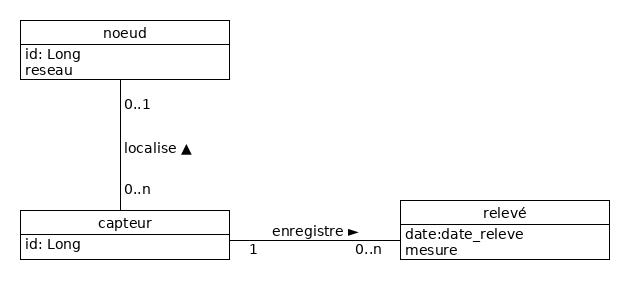
\includegraphics[width=1\textwidth]{images/uml_image1.jpg}
    \caption{modélisation UML phase 1}
    \label{fig:modélisation UML phase 1}
    \end{center}
\end{figure}

Ne Connaissant pas à l'avance quel types de capteurs on aura ni les caractéristiques de ses derniers, il nous est impossible de modéliser la table capteurs. Mais en appliquant le principe de générécité cité ci-haut, on peut alors extraire les caractéristique liés au capteurs pour les mettre dans un autre table. On appliquera le même principe pour les noeud.
\begin{figure}[!h]
   \begin{center}
        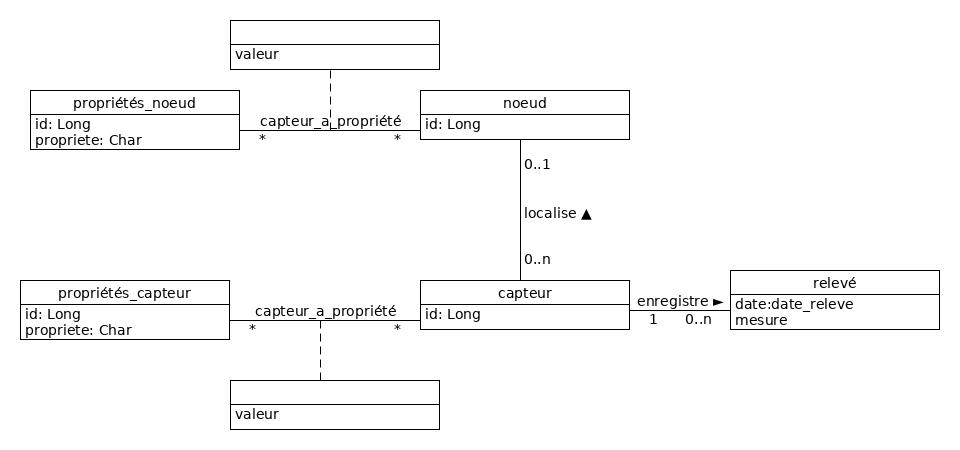
\includegraphics[width=1\textwidth]{images/uml_image2.jpg}
    \caption{modélisation UML phase 2}
    \label{fig:modélisation UML phase 2}
   \end{center}
\end{figure}



% image de la base de données
\begin{landscape}
\begin{figure}
   \begin{center}
       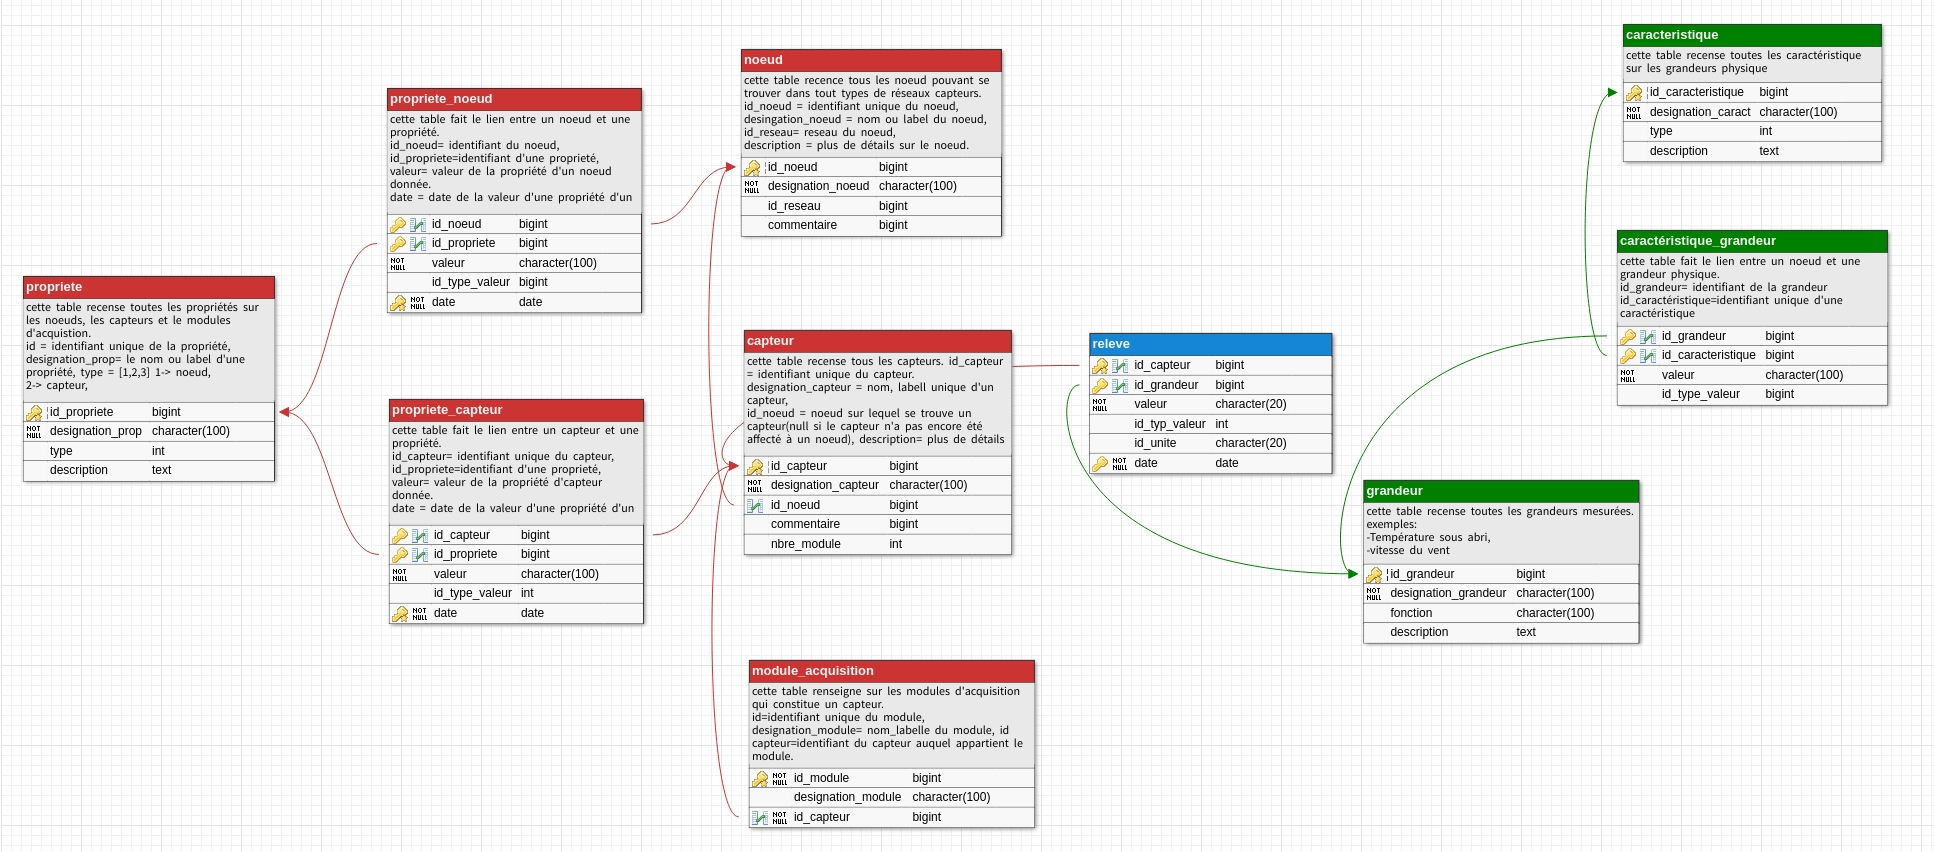
\includegraphics[width=1.8\textwidth]{images/bd_image3.jpg}
    \caption{base de données OPEROSE}
     \label{base de données OPEROSE}
   \end{center}
\end{figure}
\end{landscape}



